% !TEX root = ../Thesis.tex
\chapter{Results}

In this chapter we will address the results gained so far. Looking first at the impact of laser illumination on coherence times before examining the impact of the Stark shift on selenium donors in purified silicon and the hyperfine coupling of phosphorus donors to $^{29}$Si nuclei in natural silicon.

\section{Illumination Induced Decoherence}

\subsection{Initial Measurements}

The first step undertaken before any laser illumination occurs is to characterise the sample's $T_1$ and $T_2$ times `in the dark' at the measurement temperature. 
Experiments were performed at 8k and 7k, with typical $T_1$ and $T_2$ decays shown in figure \ref{fig:t1andt2}.
The inversion recovery has be fitted with a standard exponential decay whilst the $T_2$ decay has had a stretched exponential decay applied.
The time constants of these decays give the $T_1$ and $T_2$ times with errors in the fit used to establish errors in their values.
The stretched exponential decay of $T_2$ indicates the presence of spectral diffusion.
$T_2$ decays with dynamical decoupling applied do not have this stretch factor as they are isolated from spectral diffusion.
A problem with the results presented here is a variation in the time constant for the decay in the dark, with 2.77ms found in the high power experiments, whilst 6.4ms was found during the low power experiments. 
These results are therefore presented separately to avoid confusion.
It is possible that this is attributable to different flow rates in the helium cryostat, meaning that use of a dry cryostat, which offers much greater temperature precision, would be beneficial. 
At 7k $T_1$ was $32\pm0.1$ms and $T_2$ was unchanged.


\begin{figure}
\centering
\begin{subfigure}[b]{0.5\textwidth}
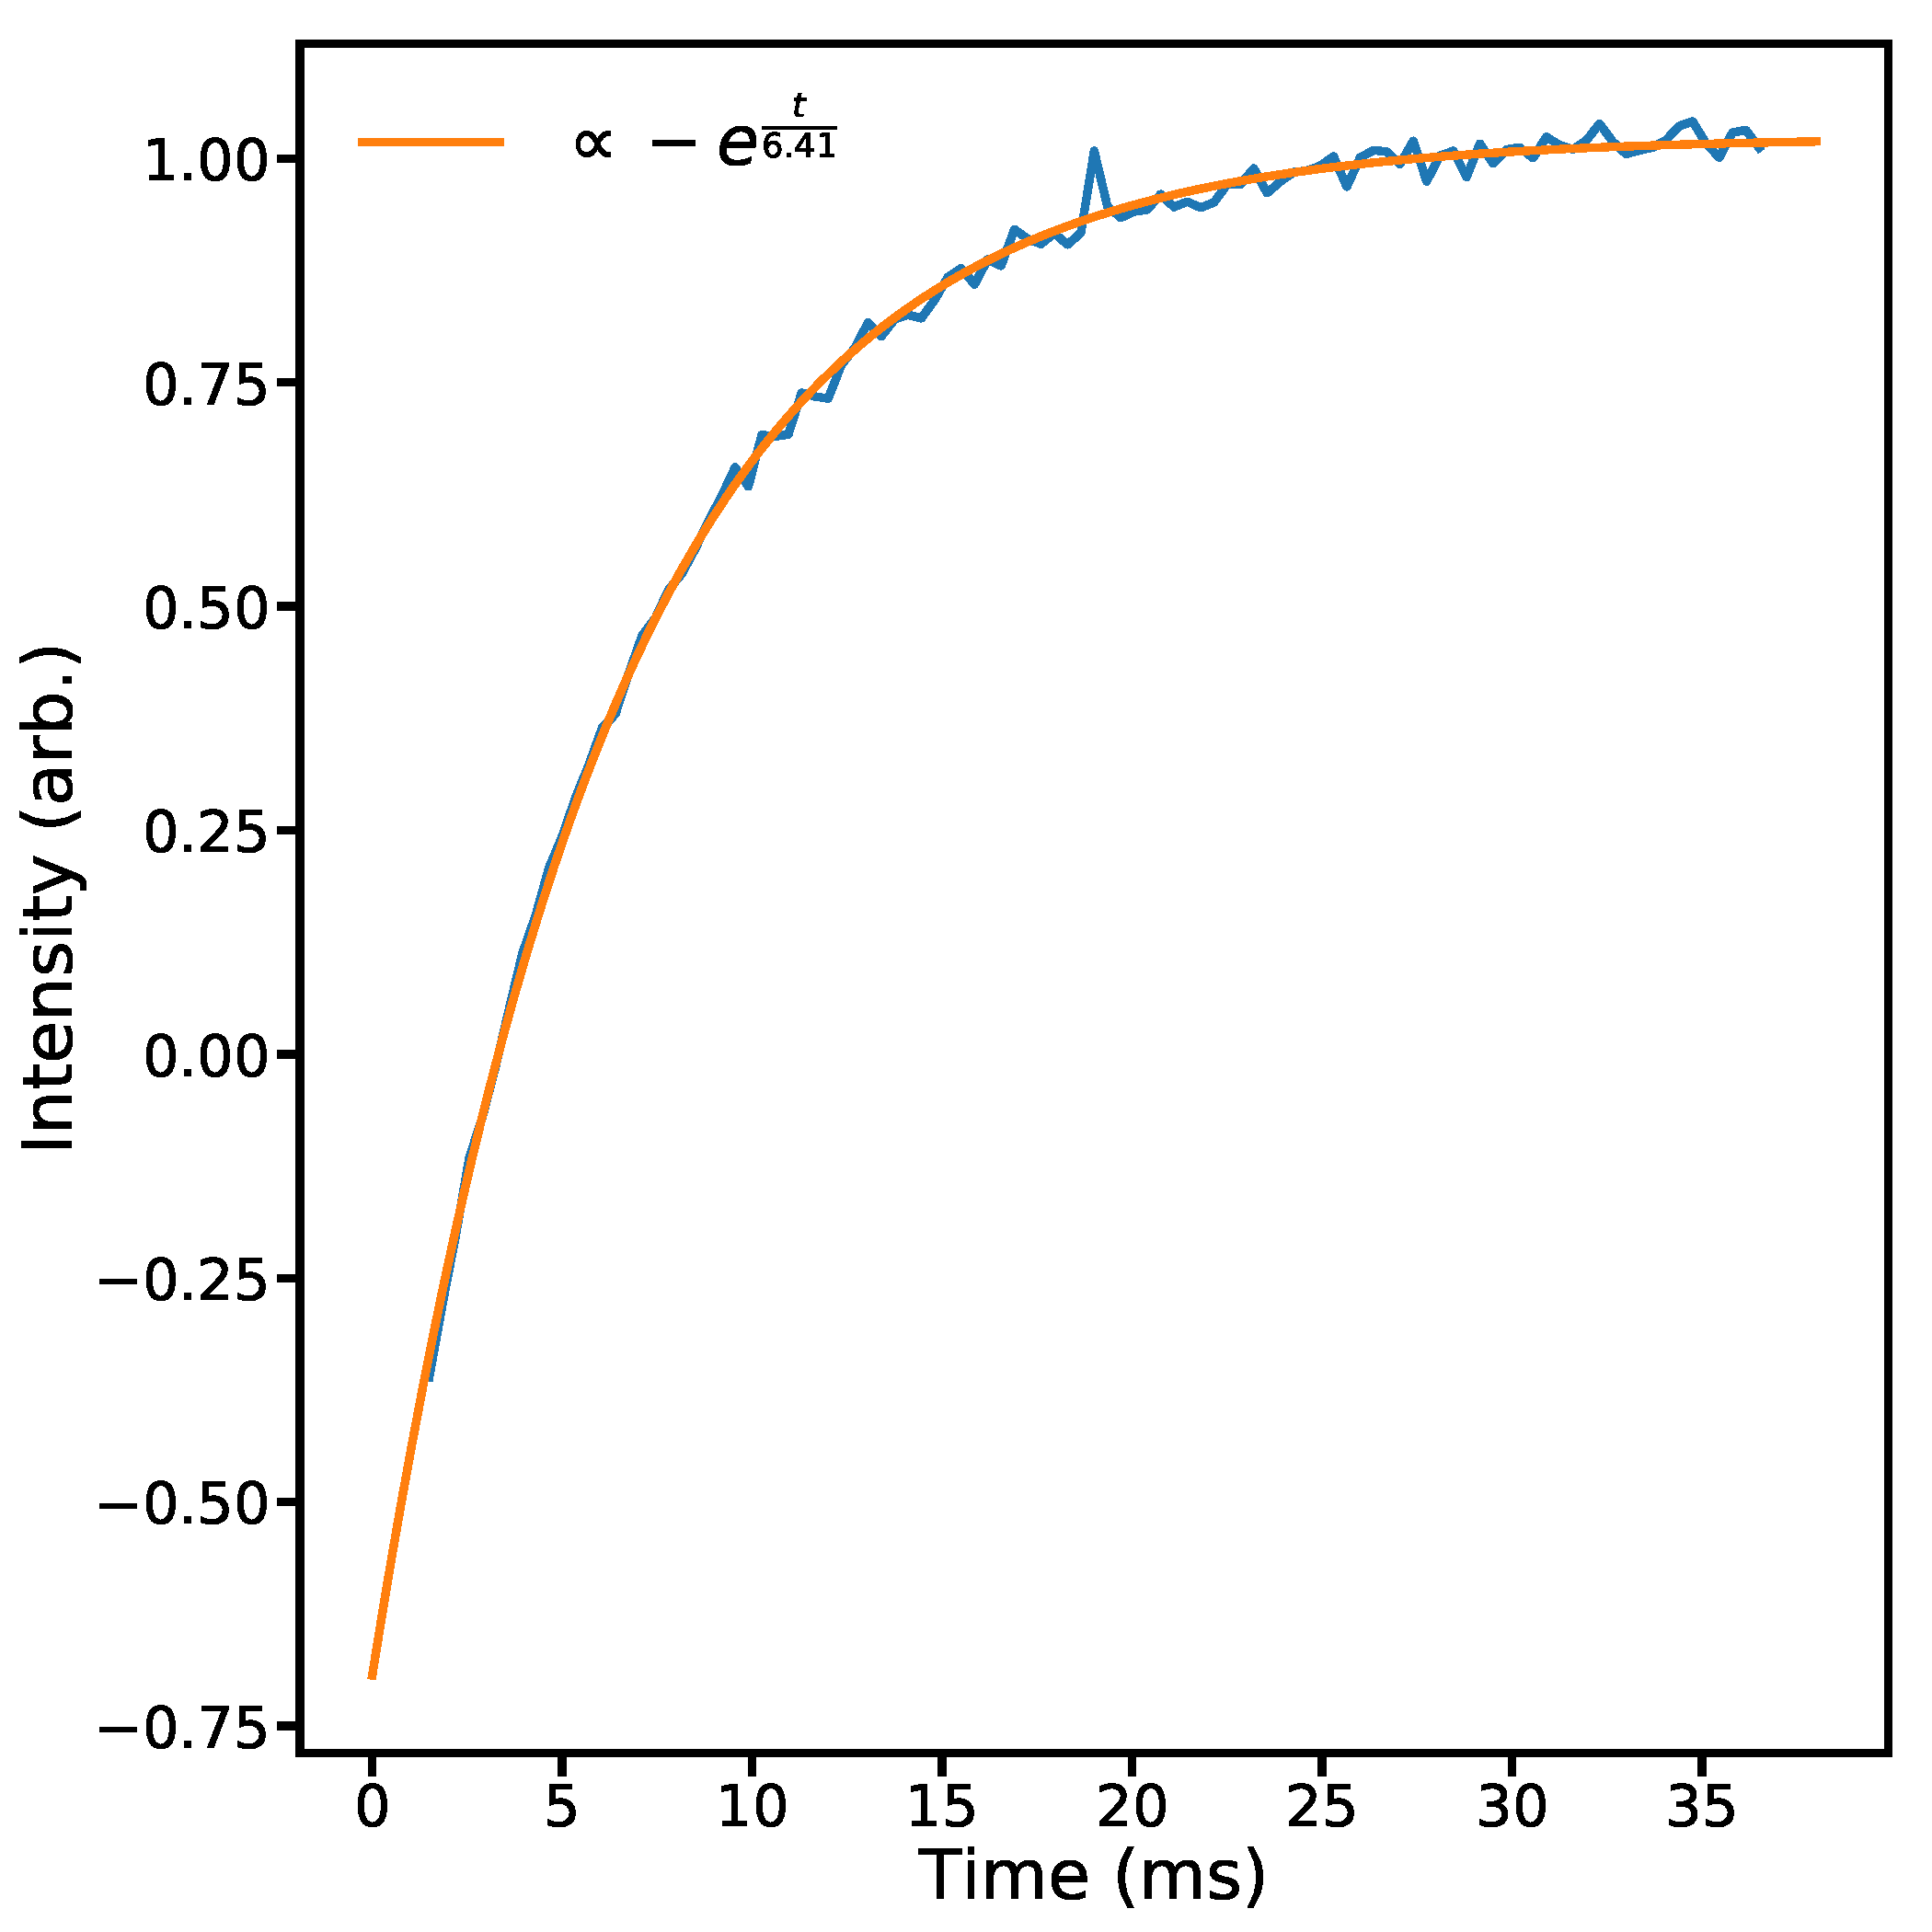
\includegraphics[width=\columnwidth]{Figures/T1Dark.pdf}{(a)}
\end{subfigure}%
\begin{subfigure}[b]{0.5\textwidth}
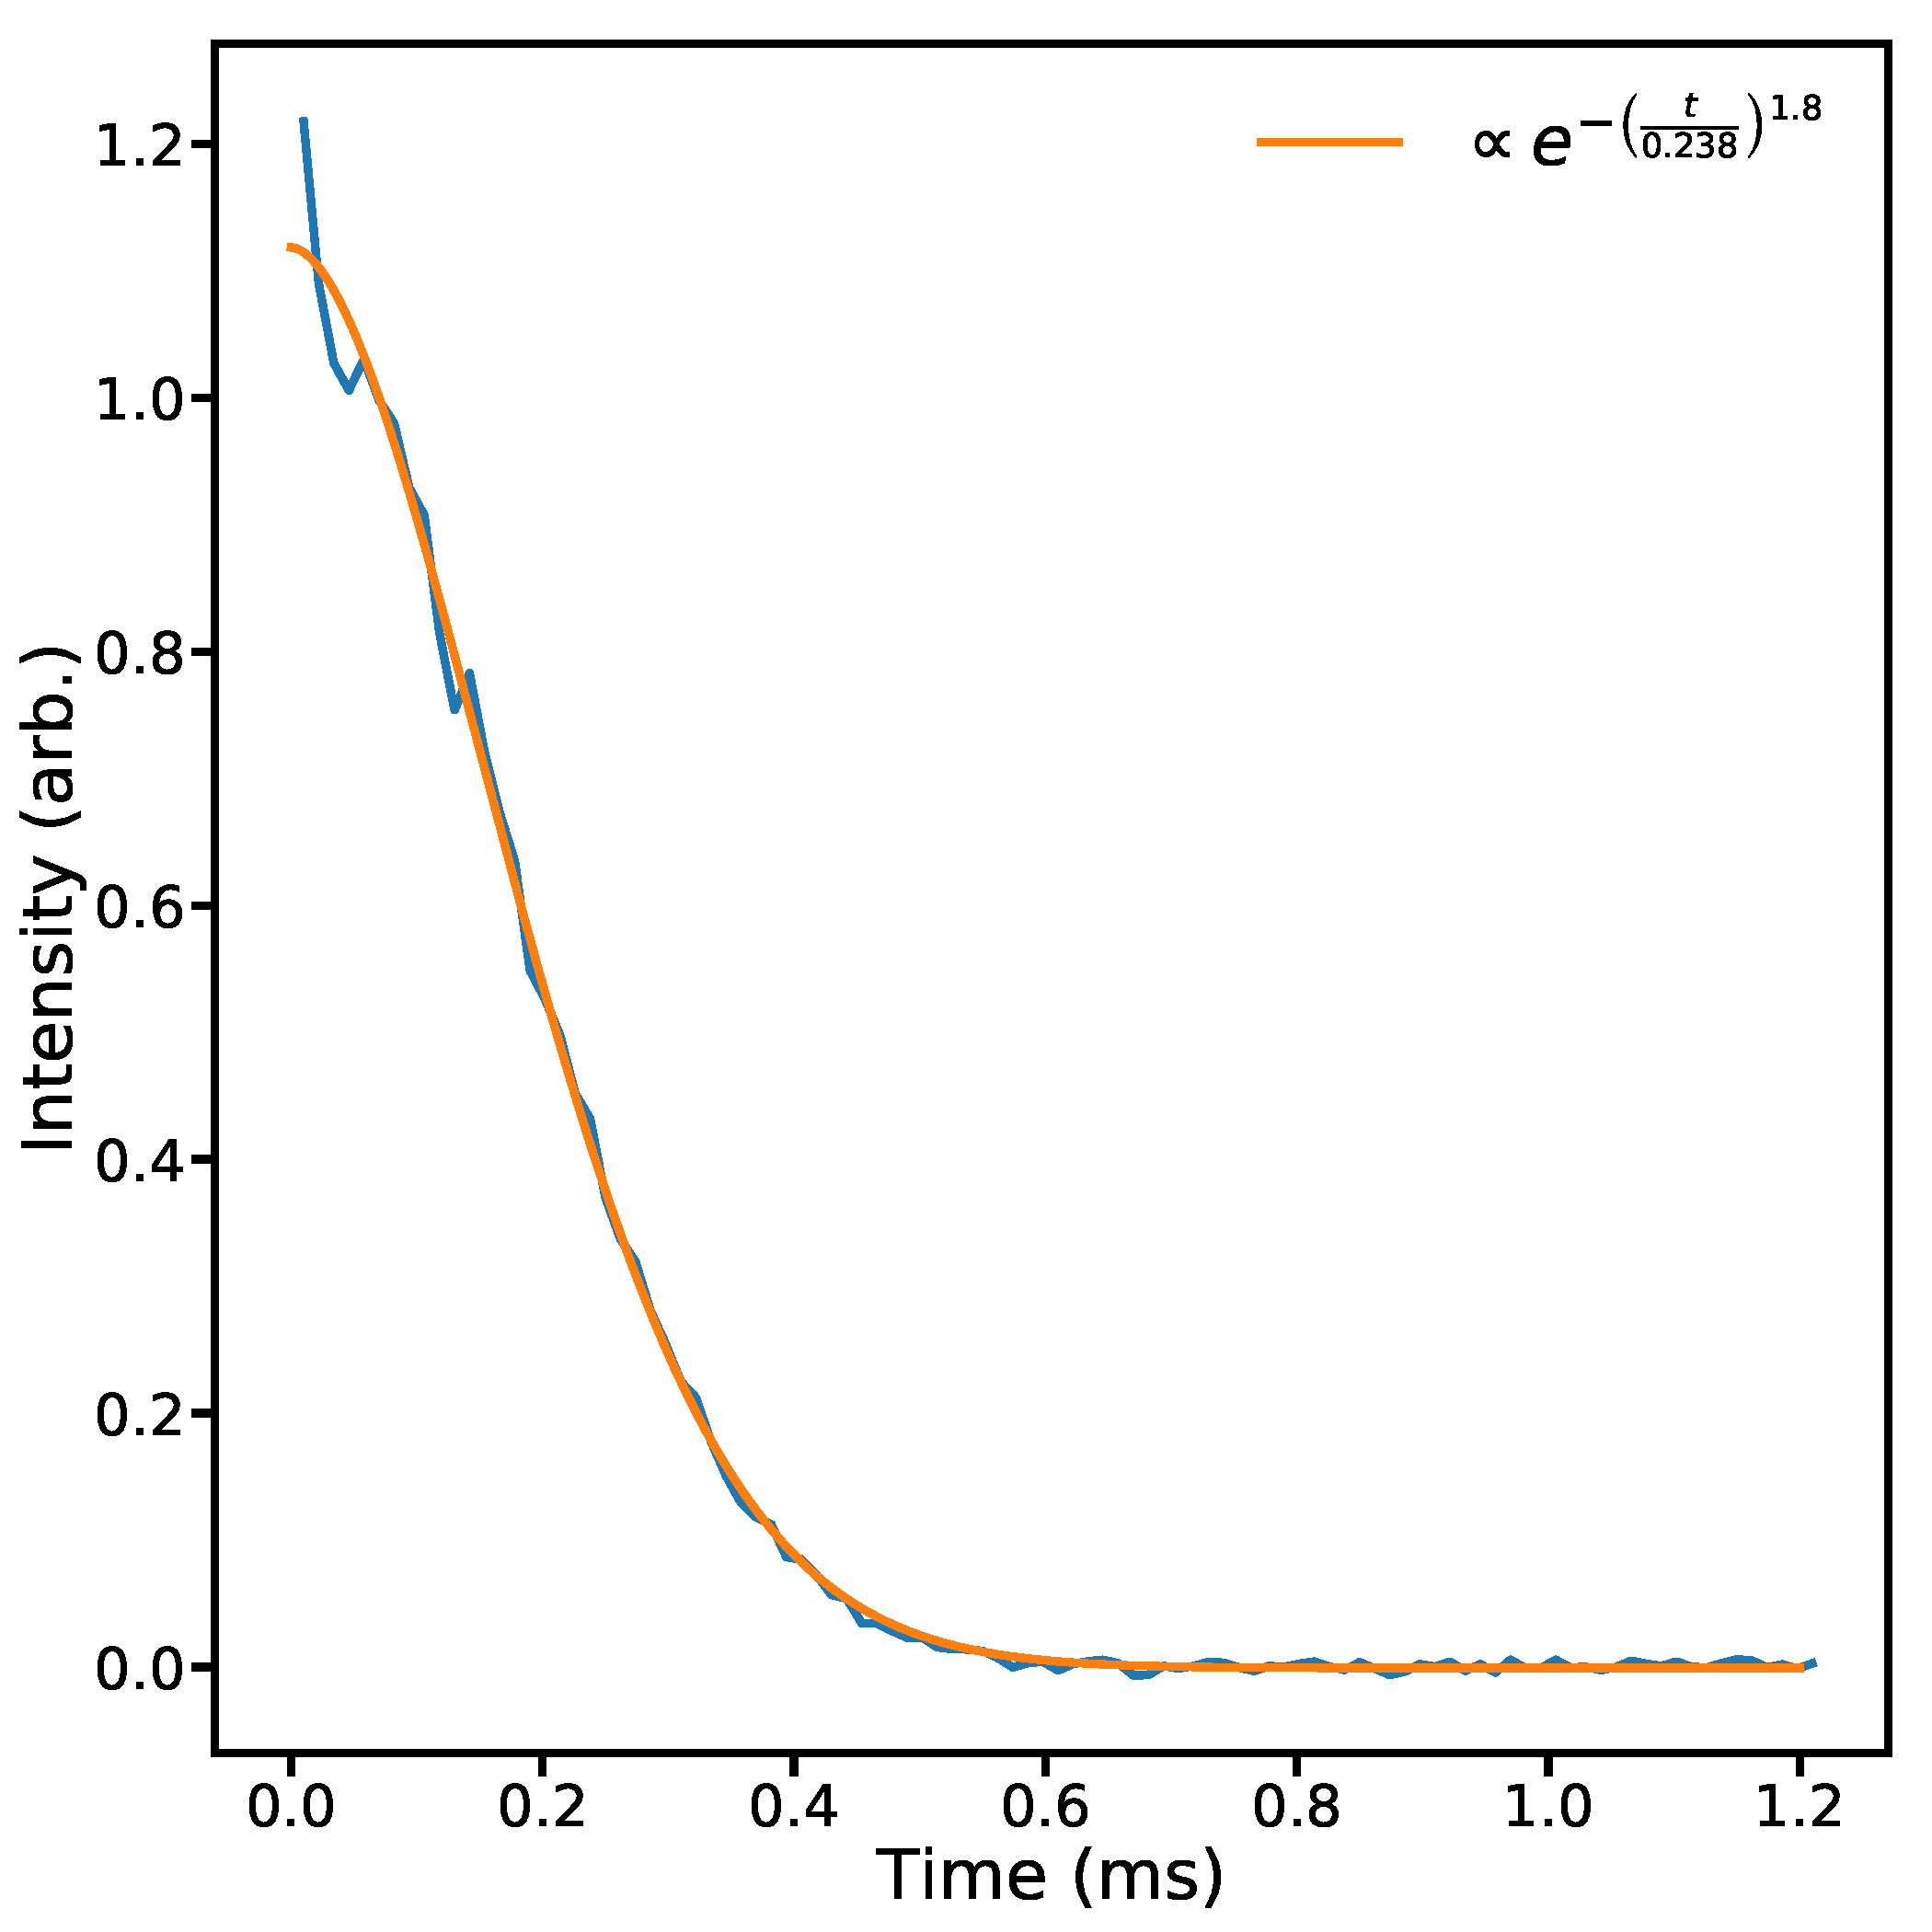
\includegraphics[width=\columnwidth]{Figures/T2Dark.pdf}{(b)}
\end{subfigure}%
\caption[$T_1$ and $T_2$ decays]{Typical $T_1$ and $T_2$ decays showing the inversion recovery for $T_1$ and the characteristic stretched exponential for $T_2$, indicating the presence of spectral diffusion.}
\label{fig:t1andt2}
\end{figure}

\subsection{Bi-Exponential Inversion Recovery}

A set of high power measurements have been taken at powers between 2mW and 130mW, at wavelengths 1060nm, 1070nm and 1080nm, and at temperatures of 7k and 8k.
At each power and wavelength 3 measurements were made: $T_1$, $T_2$ and $T_2$ whilst using a 4 $\pi$ pulse dynamical decoupling sequence - CPMG.
An initial observation is that there is a strongly bi-exponential shape to the inversion recovery, requiring a fit of the form:

\begin{equation}
a e^{\frac{t}{T_{1a}}} + b e^{\frac{t}{T_{1b}}}
\end{equation}

this is clearly seen in figure \ref{fig:biexpDec}.

\begin{figure}
\centering
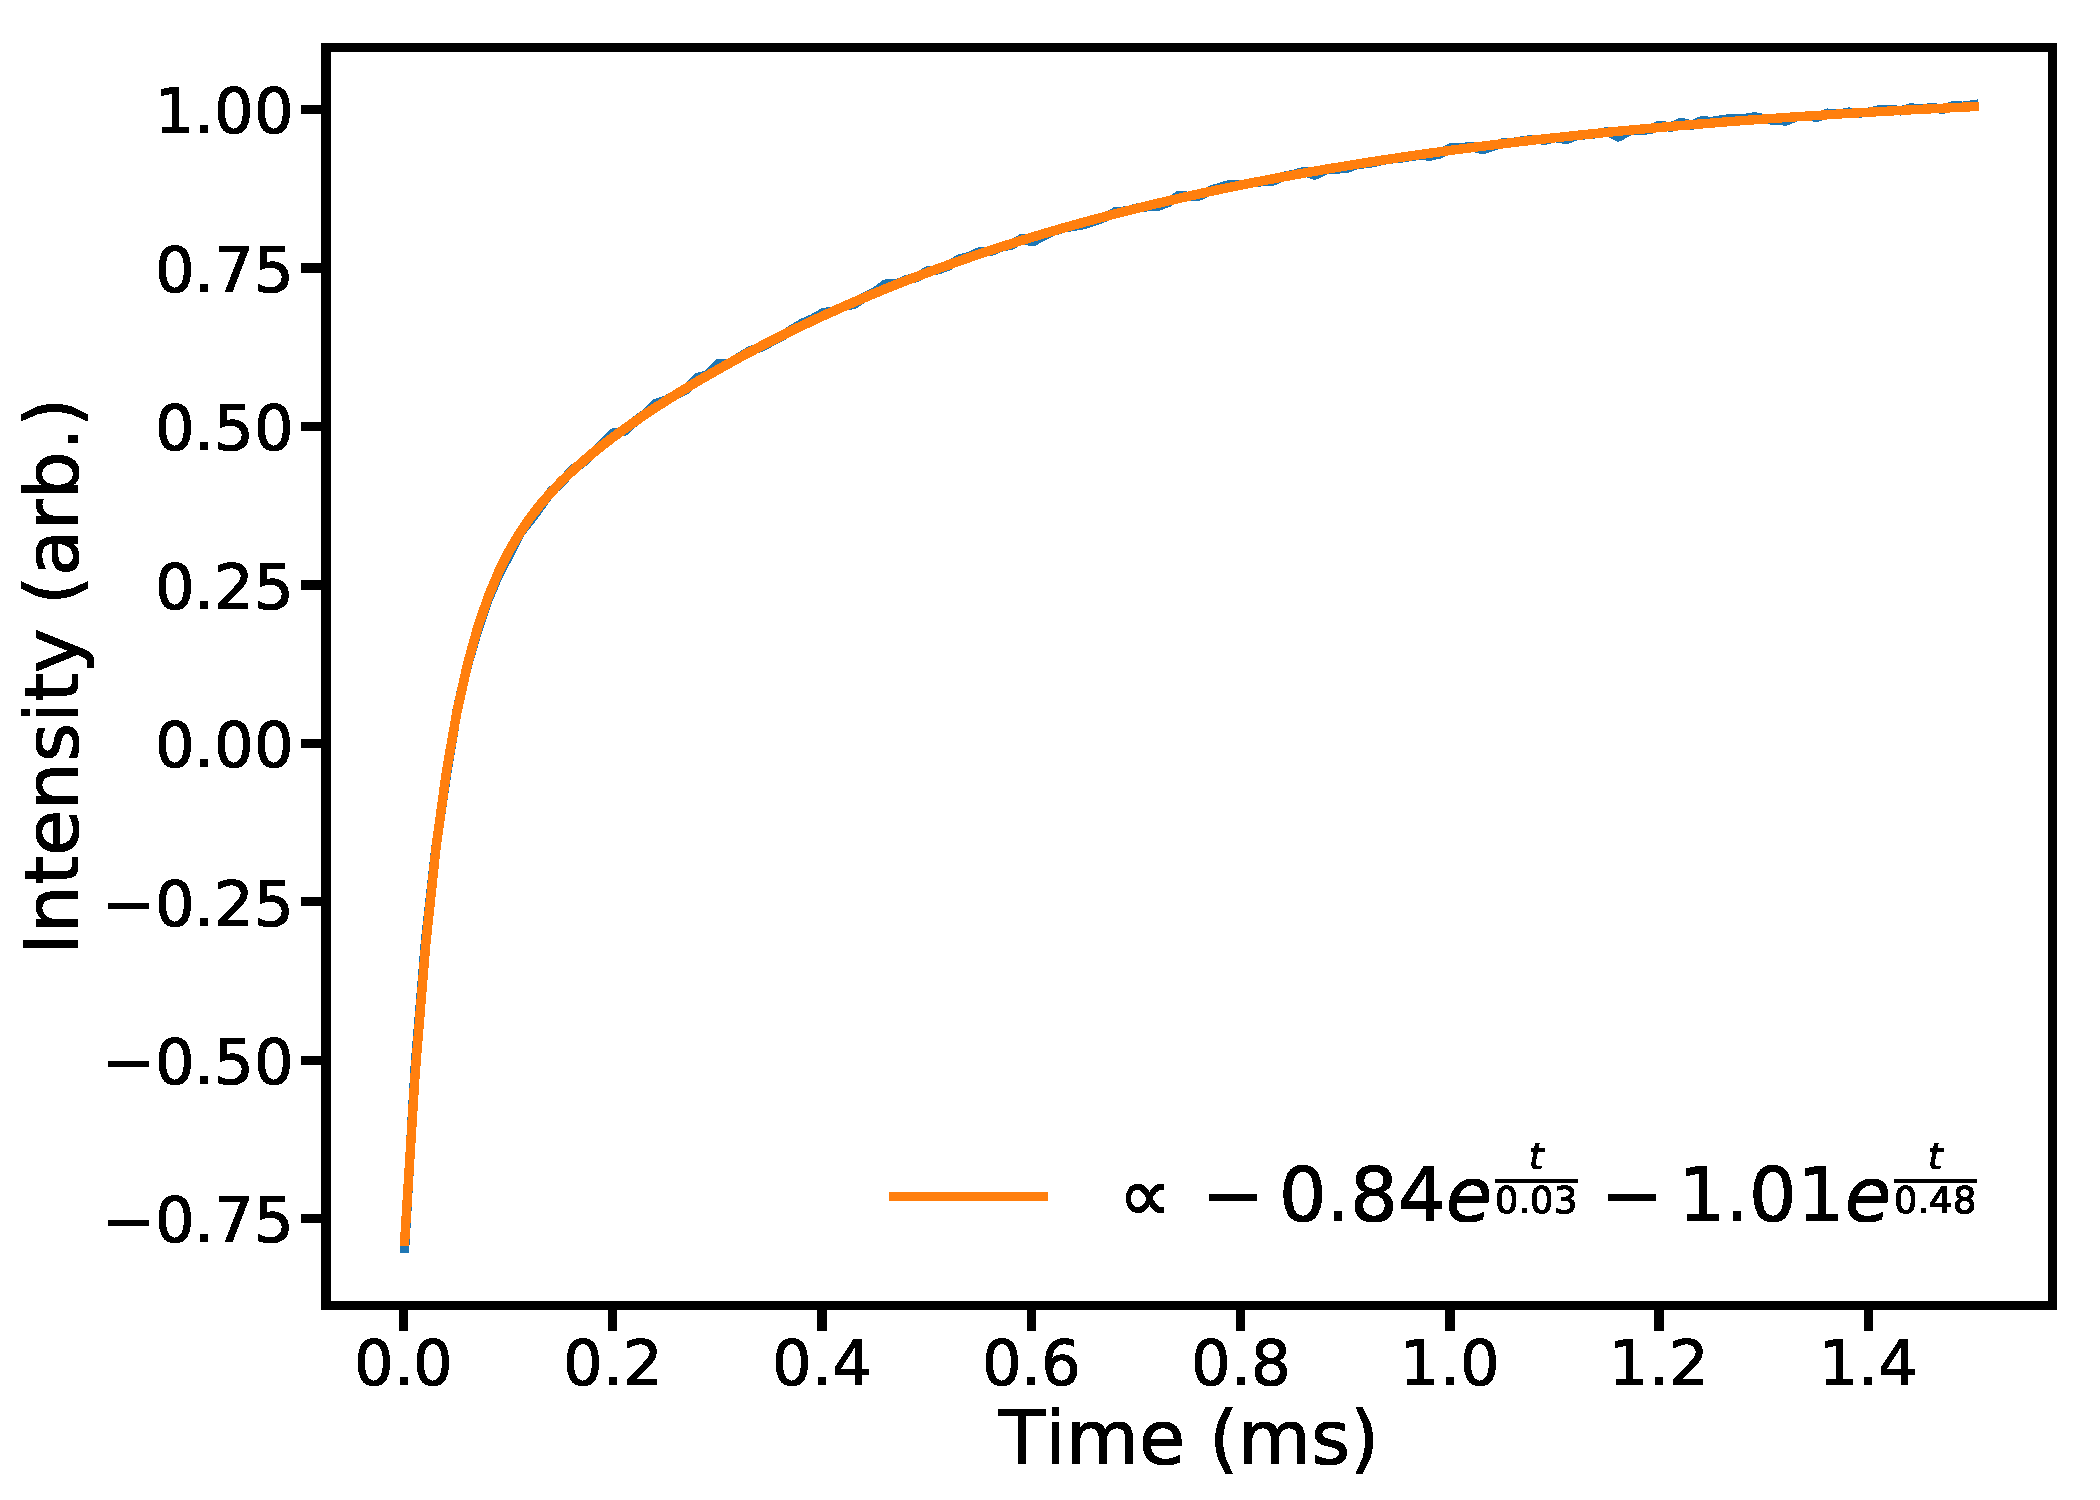
\includegraphics[width=0.8\textwidth]{Figures/T1_biExp.pdf}
\caption[Inversion recovery under laser illumination]{Inversion recovery at 8k and under 79mW illumination at 1070nm. Of note is the strongly bi-exponential nature of the decay, with two distinct time constants describing it. One significantly longer than the other. A possible explanation for this is that the laser illumination is not affecting all parts of the sample. This is not unexpected as the sample is quite large, as described in section \ref{sec:lasExps}}. 
\label{fig:biexpDec}
\end{figure}

Of the two time constants that describe the decay, one is significantly longer than the other and at low powers is close to the $T_1$ in the dark.
This suggests that there is a distribution of the illumination effect throughout the sample, with less affected parts relaxing more slowly than others. 
This becomes more obvious when comparing the two time constants over a range of powers, as seen in figure \ref{fig:T1avsT1b}.
This shows that the lower $T_1$ has a strict inverse polynomial dependence on laser power, whilst the longer $T_1$ cannot be similarly fit as it appears to saturate at lower powers.
Given this, it seems prudent when trying to determine the relationship between the incident light parameters and relaxation behaviour to use the shorter of the two time constants where a bi-exponential fit has been applied.
In the case of a set of data qubits close to the silicon surface, as is suggested in \cite{OGorman2014}, these qubits would be exposed to illumination and not shielded as appears to be the case in the long $T_1$ case.



\begin{figure}
\centering
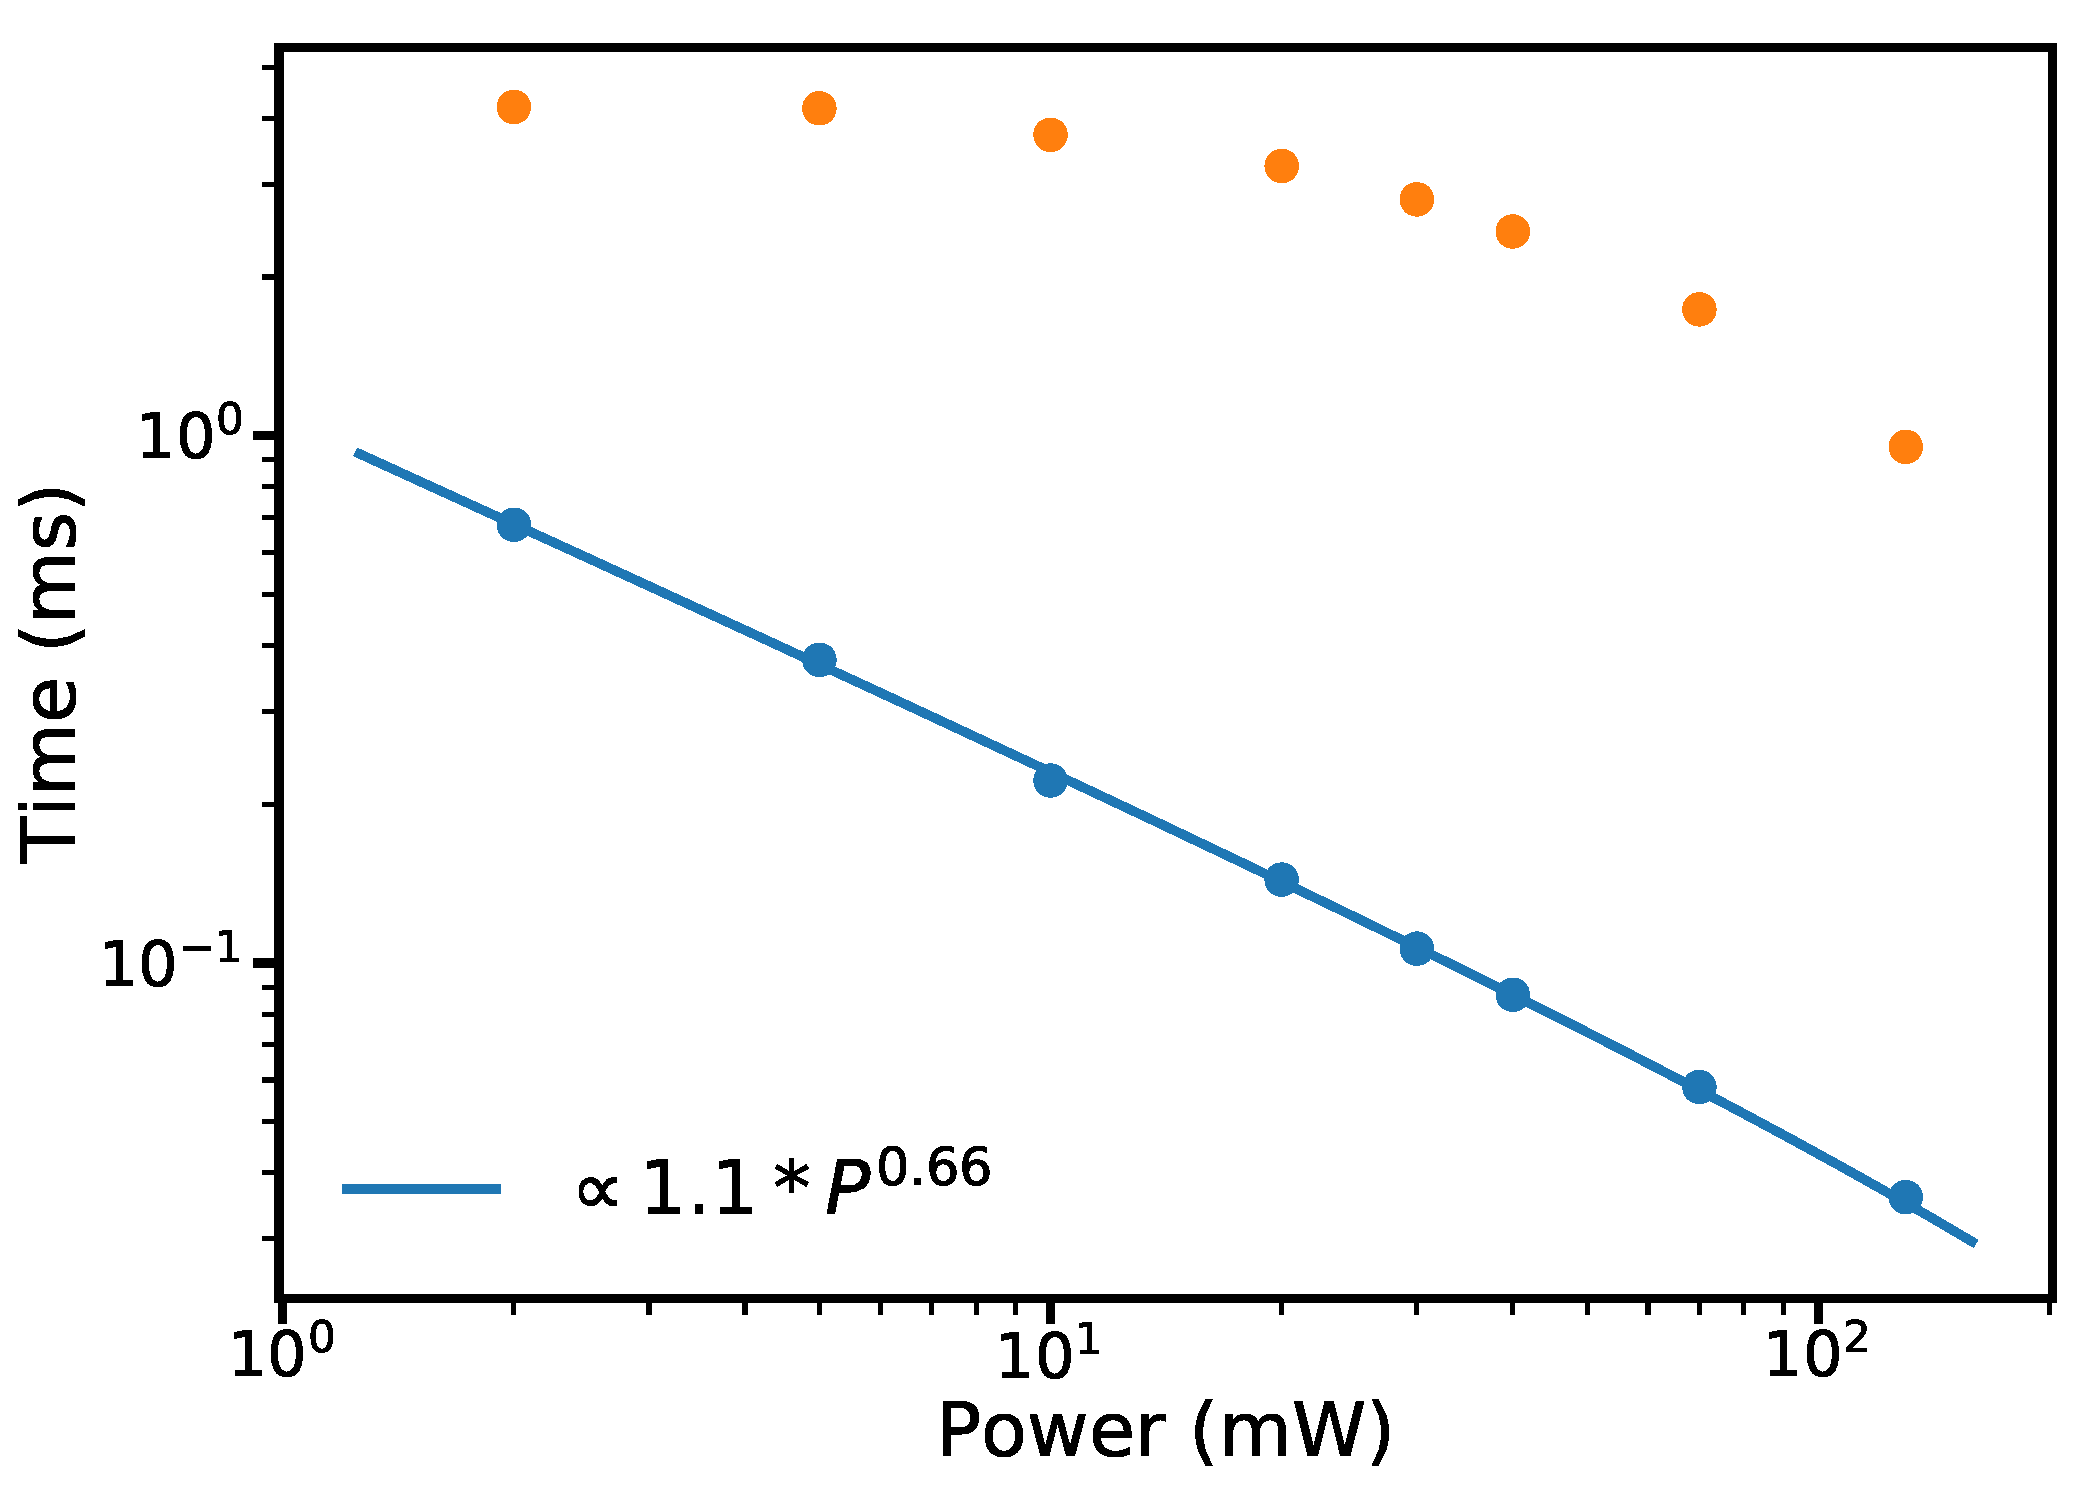
\includegraphics[width = 0.8\columnwidth]{Figures/hpT1avsT1b.pdf} 
\caption[Bi-exponential relaxation decay constants]{Figure shows the two constants for bi-exponential relaxation decay whilst under laser illumination at 1070nm and at 8k. The shorter $T_1$ constant is well fit with a $\frac{1}{P^{0.66}}$ line. A similar fit cannot be applied to the longer $T_1$ constant, which appears to demonstrate saturation behaviour at the lower illumination powers.}
\label{fig:T1avsT1b}
\end{figure}

\subsection{High Power Wavelength Comparison}
\subsubsection{Effect on $T_1$}

Measurements comparing behaviour of $T_1$, $T_2$ and dynamical decoupling $T_2$ were performed at 3 wavelengths: 1058nm, 1070nm, and 1080nm.
The lowest of these represents photon energies at approximately the band gap energy of silicon. 
As such, it would be expected that this wavelength would have a stronger effect than the other two as the free carrier generation rate would be significantly higher.
This factor has previously been postulated as the dominant process affecting relaxation rates of donor electrons.
Figure \ref{fig:wavcomparison} shows the relationship between relaxation time and laser power for three wavelengths, fitted according to $A/t^{\alpha}$. 
The power for each wavelength is $0.73\pm.002, 0.68\pm.0002$ and $0.68\pm.003$, in order of increasing wavelength.
Measurements were also taken at 2mW and 5mW but are not included here as the large error in their measurements makes them unsuitable for comparison between data sets. 
What is clear from the above graph is that there is an observable difference between the case of 1058nm illumination and the two higher wavelengths. 
This is to be expected given that 1058nm is at approximately the silicon band gap, meaning that absorption of photons will be higher and free carrier generation significantly higher than with less energetic photons.
Although the higher wavelengths have a lesser effect, there is still a strong reduction in relaxation times.
The similarity between the effects suggest that the mechanisms responsible for the increased rate do not have a strong dependence on individual photon energy once the band-gap is passed, instead the power of the incident illumination is dominant. 

\begin{figure}
\centering
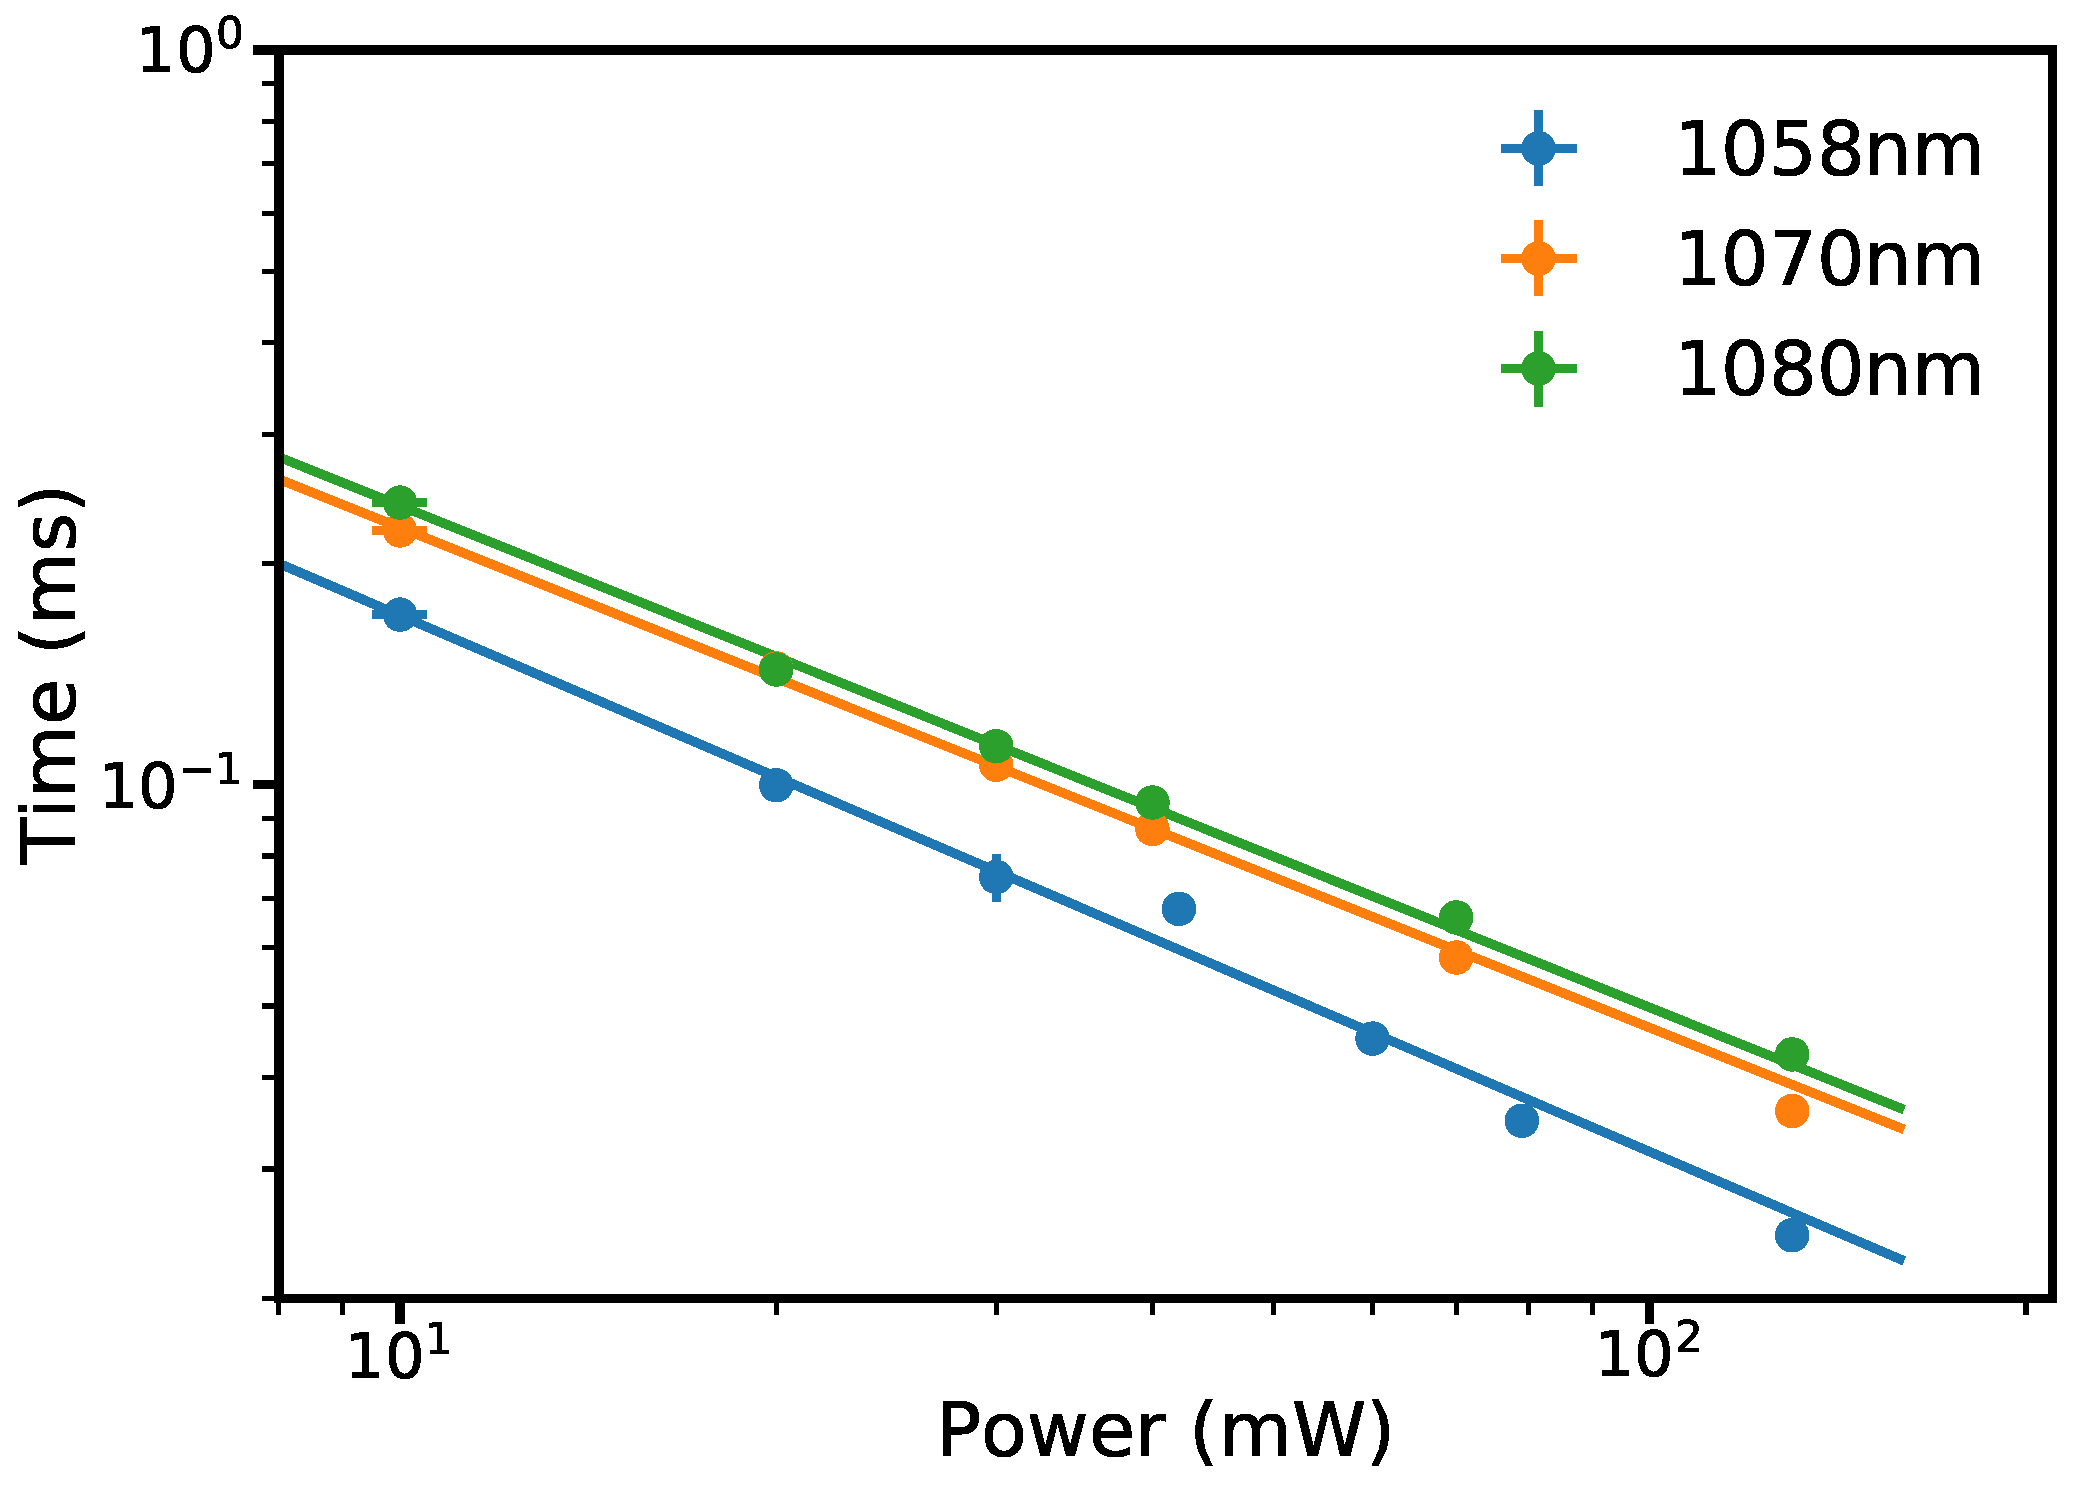
\includegraphics[width = 0.8\columnwidth]{Figures/Logwavelengthcomp.pdf}
\caption[Relaxation comparison at 8k and 1058nm, 1070nm, and 1080nm illumination]{Figure shows the relationship between laser power and relaxation time for 3 different wavelengths: 1058nm, 1070nm and 1080nm.}
\label{fig:wavcomparison}
\end{figure}

The impact of illumination on relaxation rates observed here is in line with predictions.
Increased wavelength results in a slower relaxation rate at equivalent powers, with a more significant change being observed as the silicon band gap energy is crossed.
Relaxation rates follow a $a/P^{\alpha}$

\subsubsection{Effect on $T_2$}

Whilst the $T_1$ time is important for quantum information processing, as it ultimately limits computation time, $T_2$ is in most cases the limiting factor in qubit coherence.
The mechanisms that limit $T_2$ in spins were discussed in section \ref{sec:litdecoherence}.
Of particular worry is that a significant number of free electrons in the silicon conduction band could create time dependent magnetic fields at the observed donor spins. 
If this is the case then there could be an impact on the $T_2$ time beyond the effect of reduced $T_1$.
Figure \ref{fig:t1vst2wav} shows how $T_1$ and $T_2$ vary with laser power for 1058nm and 1070nm.
What is clear in both cases is that there does not appear to be a significant effect beyond $T_2$ being limited by $T_1$.
In both graphs it is clear at the lower powers that $T_2$ is beginning to saturate to the value in the dark of $220\mu$s.
The fact that there is no clear difference between the effects in the 1058nm case and the 1070nm case is interesting. 
It suggests that, although there is clearly a greater magnitude of effect in the lower wavelength case, if the mechanism is different then it has no impact on $T_2$ above and beyond the extra $T_1$ limitation.



\begin{figure}
\centering
\begin{subfigure}[b]{0.5\columnwidth}
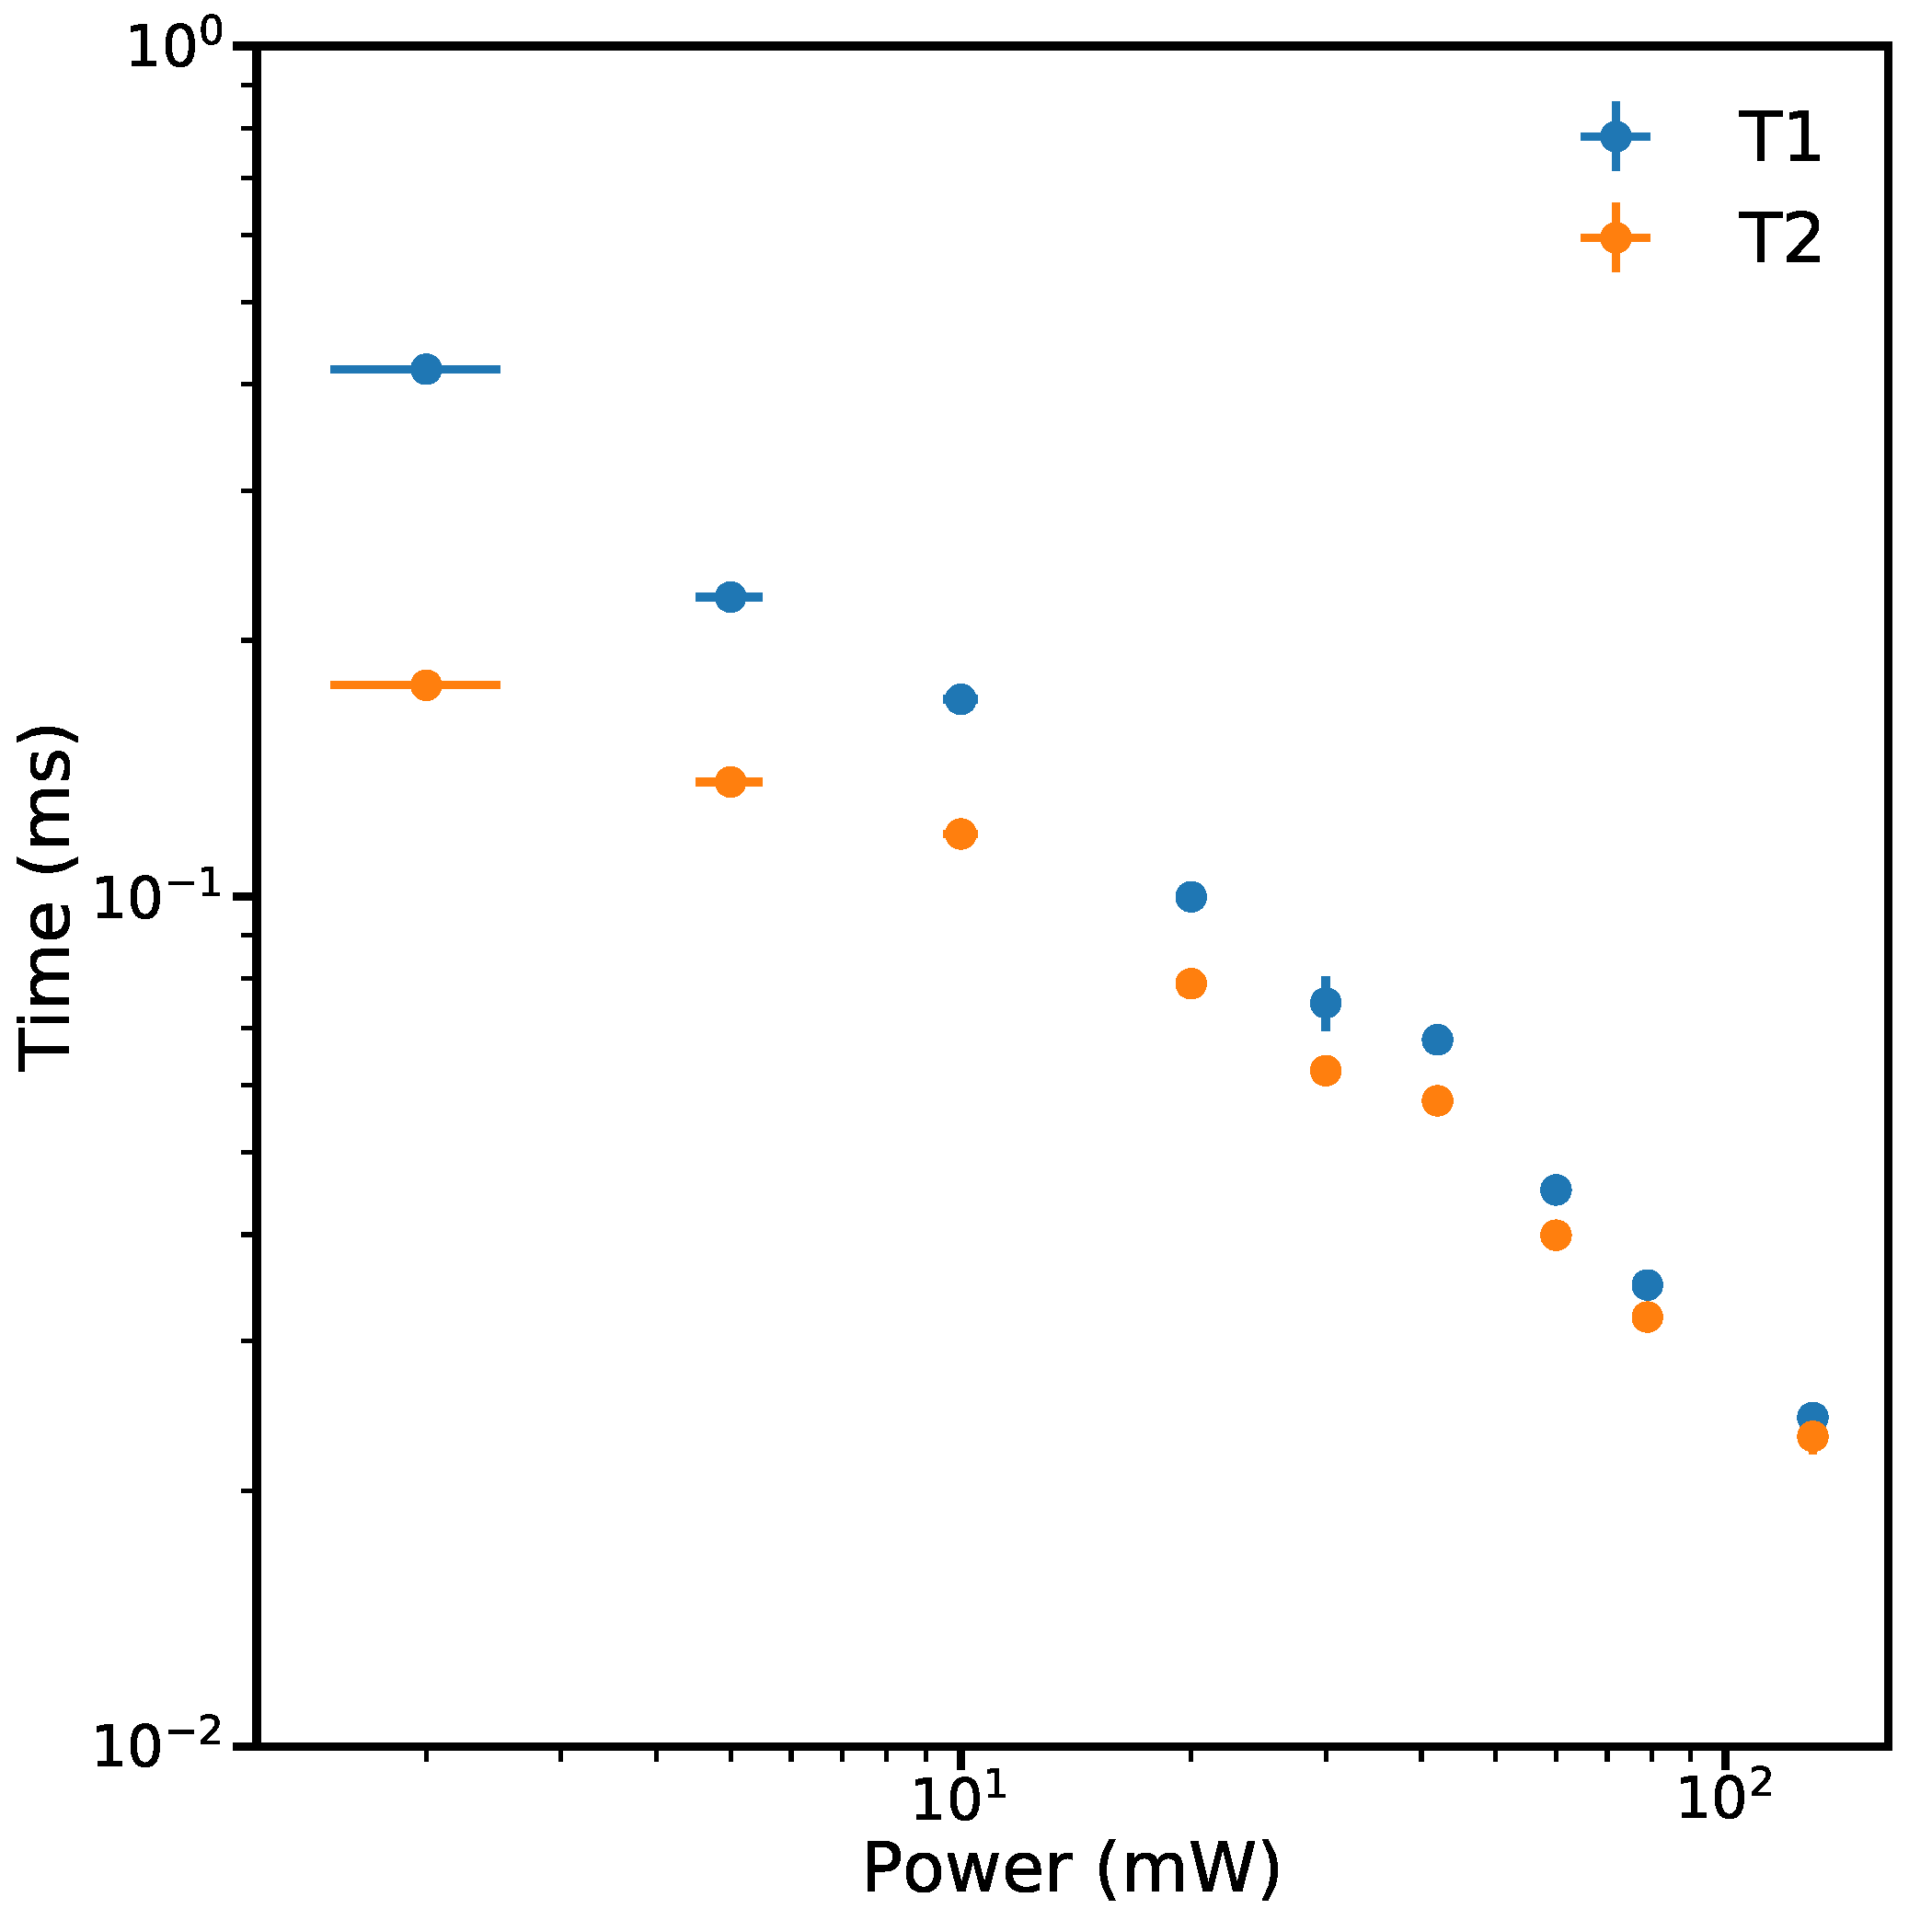
\includegraphics[width = \columnwidth]{Figures/8kT1vsT21058.pdf}{(a)}
\end{subfigure}%
\begin{subfigure}[b]{0.5\columnwidth}
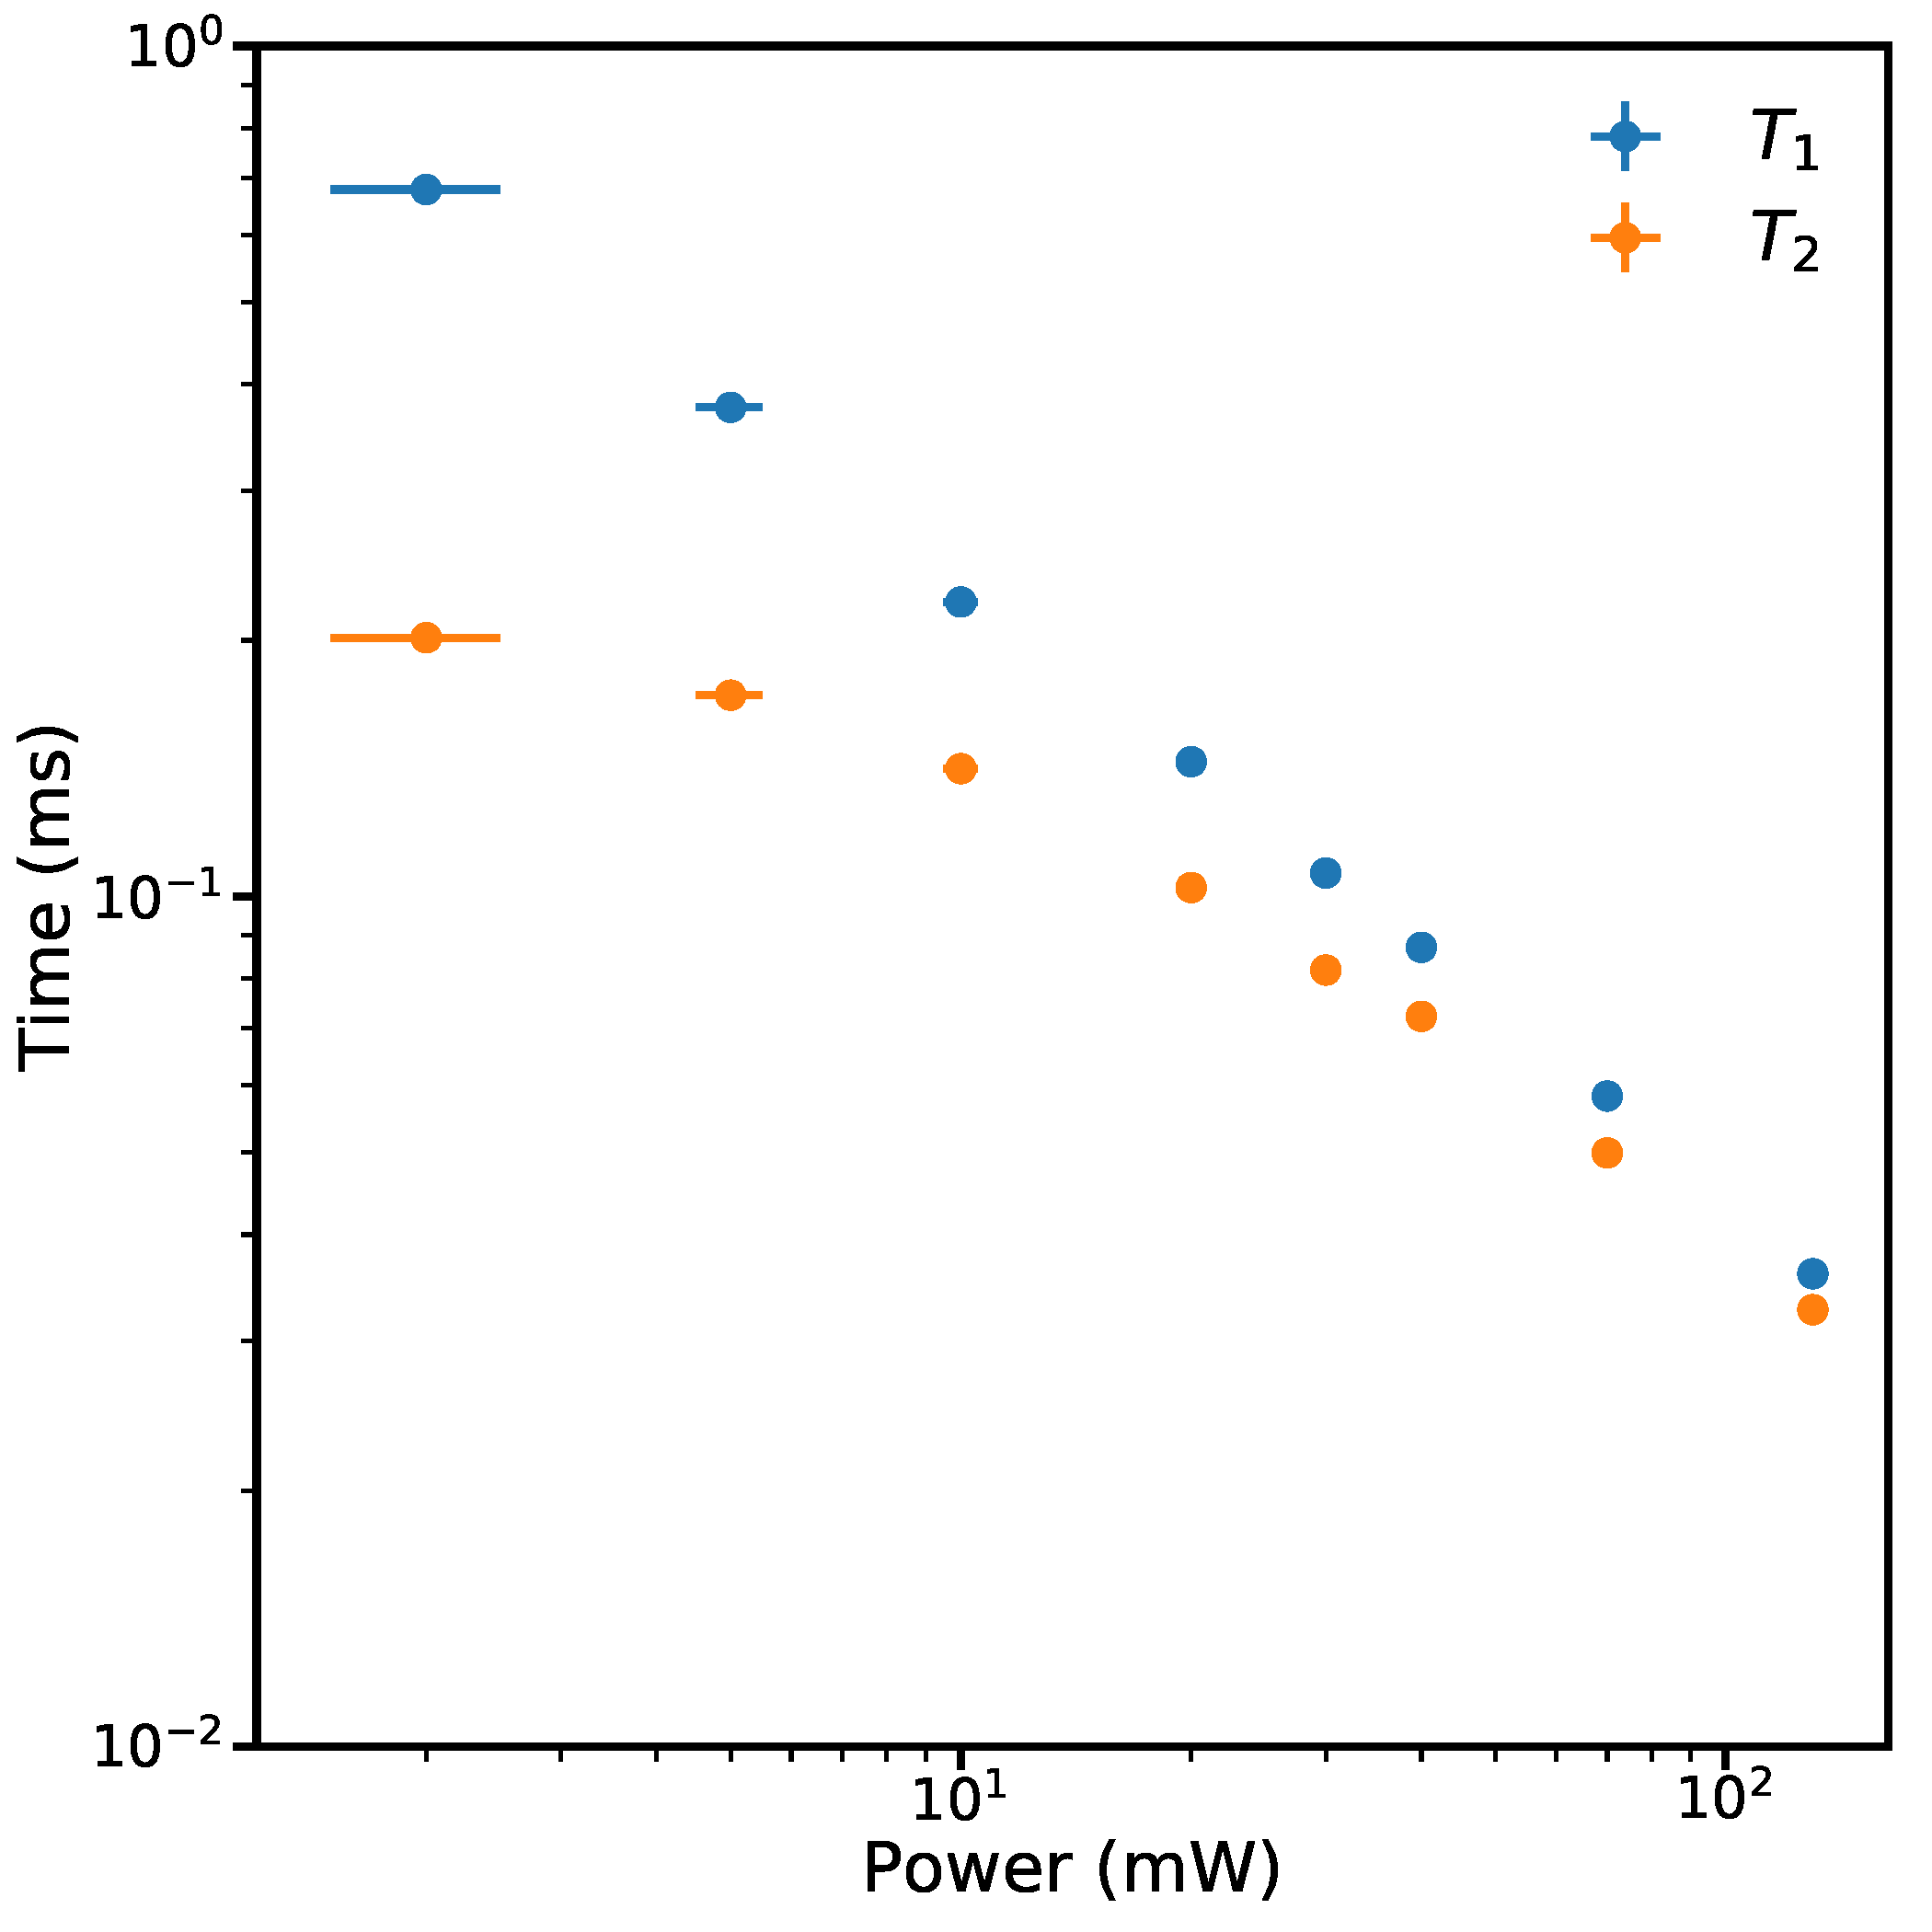
\includegraphics[width=\columnwidth]{Figures/T1vsT11070.pdf}
\end{subfigure}%
\caption[$T_1$ vs $T_2$ for 1058nm and 1070nm]{Figures showing how both $T_1$ and $T_2$ vary with laser power, presented on the same scale for ease of comparison. At high powers $T_1$ is observed to be close to $T_2$, essentially limiting it. }
\label{fig:t1vst2wav}
\end{figure}
